% !TeX root = ../main.tex
\chapter{Unidad 5: Análisis frecuencial de señales acústicas}
\label{chap:unidad-5}

\section{Propósito y resultados de aprendizaje}
\label{sec:u5-proposito}

Una señal acústica puede observarse como una variación de presión a lo largo
del tiempo. Esa representación permite reconocer duración, transitorios,
periodicidad y cambios de amplitud. Sin embargo, no siempre permite identificar
con facilidad qué oscilaciones contribuyen a la forma registrada. El análisis
frecuencial ofrece otra descripción de la misma señal: informa cómo se
distribuyen sus componentes según la frecuencia.

Esta unidad introduce las herramientas necesarias para pasar de una descripción
temporal a una descripción frecuencial y para interpretar filtros, bandas y
mediciones sonométricas. Al finalizar, se espera que el estudiante pueda:

\begin{itemize}
    \item distinguir señales periódicas, aperiódicas y transitorias a partir de
    su comportamiento temporal;
    \item relacionar una señal temporal con sus espectros de magnitud y fase;
    \item explicar la serie y la transformada de Fourier como representaciones
    matemáticas, no como mecanismos que crean componentes físicas;
    \item diferenciar el espectro de una señal de la respuesta en frecuencia de
    un sistema;
    \item distinguir frecuencia fundamental, armónico, parcial y sobretono sin
    identificar automáticamente la fundamental con el componente de mayor
    amplitud;
    \item calcular resolución frecuencial, límites y ancho de bandas de octava
    y tercio de octava;
    \item interpretar las respuestas de filtros pasa bajos, pasa altos, pasa
    banda y elimina banda;
    \item diferenciar ponderación frecuencial, filtrado de una señal y filtrado
    audiométrico;
    \item describir la cadena funcional de un sonómetro y distinguir nivel
    equivalente, nivel máximo y nivel pico.
\end{itemize}

\section{Conocimientos previos}
\label{sec:u5-conocimientos-previos}

La Unidad~\ref{chap:unidad-3} introdujo período, frecuencia, fase,
sinusoides y superposición. La Unidad~\ref{chap:unidad-4} definió presión
acústica, valor eficaz, señal compleja y niveles logarítmicos. En particular,
conviene recordar que:

\begin{itemize}
    \item la frecuencia \(f\) se mide en hertz (\(\text{Hz}\));
    \item el tiempo \(t\) y el período \(T\) se miden en segundos
    (\(\text{s}\));
    \item la presión acústica instantánea \(p(t)\) se mide en pascales
    (\(\text{Pa}\));
    \item un nivel de presión sonora \(L_p\) es una relación logarítmica y no
    es sinónimo de intensidad, sonoridad ni nivel de audición;
    \item la frecuencia es una magnitud física, mientras que la altura tonal o
    \emph{pitch} es un atributo perceptual.
\end{itemize}

\section{Dos descripciones de una misma señal}
\label{sec:u5-tiempo-frecuencia}

Considérese la presión acústica \(p(t)\), en pascales, registrada por un
micrófono calibrado. En el \textbf{dominio temporal}, el eje horizontal
representa el tiempo \(t\), en segundos, y el eje vertical representa la
presión instantánea. Esta vista permite observar cuándo comienza y termina un
evento, cómo cambia su amplitud y si existe repetición.

En el \textbf{dominio frecuencial}, el eje horizontal representa la frecuencia
\(f\), en hertz. El eje vertical debe identificarse con cuidado: puede
representar amplitud espectral, magnitud de una transformada, potencia por
banda, densidad espectral u otra cantidad. Una ordenada expresada en decibeles
también debe declarar la magnitud de origen, la referencia y la normalización.
Por lo tanto, no corresponde llamar ``intensidad'' a cualquier eje espectral.

Las dos representaciones describen la misma señal desde perspectivas
complementarias. La representación temporal no ``contiene menos información''
por no mostrar picos de frecuencia; la representación frecuencial reorganiza
esa información mediante un modelo matemático.

La figura~\ref{fig:u5-tiempo-magnitud-fase} aplica las dos lecturas a la presión
del ejemplo que se resolverá más adelante. Además muestra que la fase requiere
su propia representación: no queda contenida en la altura de las líneas del
espectro de magnitud.

\begin{figure}[htbp]
    \centering
    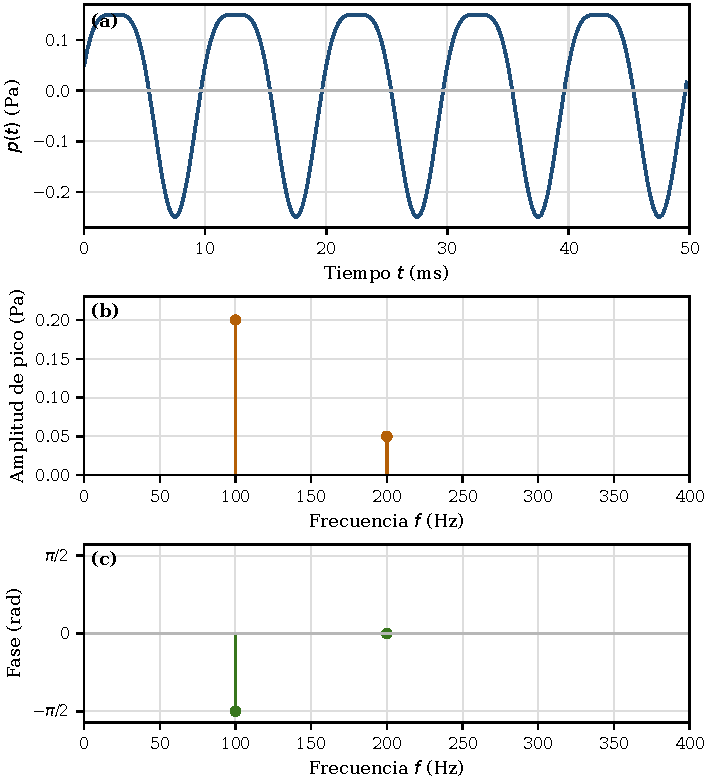
\includegraphics[width=0.96\textwidth]
        {figures/generated/unidad-5/tiempo-magnitud-fase.pdf}
    \caption{Una misma presión acústica teórica en tres representaciones:
    (a)~registro temporal; (b)~amplitud de pico de cada componente de la DFT;
    y (c)~fase de esas componentes. La señal se construyó con tonos de
    \(100\,\text{Hz}\) y \(200\,\text{Hz}\), se muestreó a
    \(f_s=4000\,\text{Hz}\) durante \(T_\mathrm{obs}=0{,}050\,\text{s}\) y se
    analizó sin ventana adicional, por lo que
    \(\Delta f=20\,\text{Hz}\). Datos sintéticos calculados; no constituyen una
    medición. Elaboración propia.}
    \label{fig:u5-tiempo-magnitud-fase}
\end{figure}

\subsection{Señales periódicas, aperiódicas y transitorias}
\label{sec:u5-periodicas-aperiodicas}

Una señal \(x(t)\), que puede representar presión, tensión eléctrica u otra
magnitud, es \textbf{periódica} si existe un intervalo positivo \(T\), medido
en segundos, tal que

\begin{equation}
    x(t+T)=x(t)
    \label{eq:u5-periodicidad}
\end{equation}

para todo instante \(t\) del modelo. El menor período positivo que satisface
esta relación se denomina período fundamental y se representará mediante
\(T_0\). Su frecuencia fundamental es

\begin{equation}
    f_0=\frac{1}{T_0},
    \label{eq:u5-fundamental-periodo}
\end{equation}

donde \(f_0\) se mide en hertz.

Una señal es \textbf{aperiódica} cuando no repite exactamente un mismo patrón
con un período fundamental. Una frase hablada completa, un golpe y una
realización de ruido son ejemplos posibles. Una señal \textbf{transitoria}
presenta cambios asociados con un comienzo, un final o una modificación
rápida. Las categorías no son excluyentes en registros reales: una vocal
sostenida puede ser aproximadamente periódica durante un intervalo y contener
transitorios al inicio y al final.

\section{Herramientas de Fourier}
\label{sec:u5-fourier}

Las herramientas de Fourier representan una señal mediante sinusoides o,
equivalentemente, mediante exponenciales complejas. Esta descomposición no
implica que un dispositivo físico separe necesariamente el sonido en piezas
independientes. Es una forma de describir y calcular propiedades de la señal.

\subsection{Serie de Fourier}
\label{sec:u5-serie-fourier}

Para una señal periódica \(x(t)\) con período fundamental \(T_0\), una forma
trigonométrica de la serie de Fourier es

\begin{equation}
    x(t)=\frac{a_0}{2}
    +\sum_{n=1}^{\infty}
    \left[
        a_n\cos(2\pi n f_0t)
        +b_n\sin(2\pi n f_0t)
    \right],
    \label{eq:u5-serie-fourier}
\end{equation}

donde \(f_0=1/T_0\), \(n\) es un entero positivo y los coeficientes
\(a_0\), \(a_n\) y \(b_n\) poseen la misma unidad que \(x(t)\). Para la
convención de la ecuación~\eqref{eq:u5-serie-fourier}, se calculan sobre un
período mediante

\begin{align}
    a_n&=\frac{2}{T_0}\int_{0}^{T_0}
        x(t)\cos(2\pi n f_0t)\,dt,
        \label{eq:u5-coef-an}\\
    b_n&=\frac{2}{T_0}\int_{0}^{T_0}
        x(t)\sin(2\pi n f_0t)\,dt.
        \label{eq:u5-coef-bn}
\end{align}

Para \(n=0\), la primera de estas expresiones determina \(a_0\) al reemplazar
el coseno por uno. El término \(a_0/2\) representa el valor medio de la señal.
Los términos con frecuencias \(nf_0\) representan componentes armónicas. Una
suma con pocos términos produce una aproximación; al agregar términos puede
reproducirse con mayor detalle la forma temporal dentro de las condiciones de
validez de la serie.

La figura~\ref{fig:u5-serie-fourier-progresiva} permite observar esa
aproximación de manera progresiva. Las oscilaciones que permanecen cerca de cada
discontinuidad no representan ruido de medición: corresponden al comportamiento
de la suma parcial y se asocian con el fenómeno de Gibbs.

\begin{figure}[htbp]
    \centering
    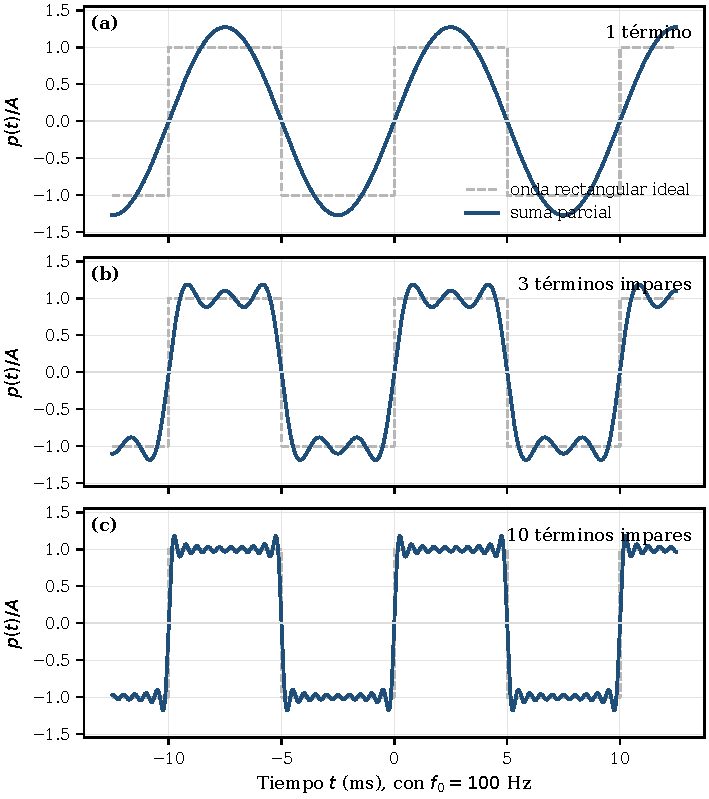
\includegraphics[width=0.96\textwidth]
        {figures/generated/unidad-5/serie-fourier-progresiva.pdf}
    \caption{Aproximación progresiva de una onda rectangular normalizada de
    frecuencia fundamental \(f_0=100\,\text{Hz}\). Se suman uno, tres y diez
    términos impares de
    \(\frac{4}{\pi}\sum_{m=0}^{M-1}
    \sin[2\pi(2m+1)f_0t]/(2m+1)\).
    Al aumentar \(M\), la suma reproduce mejor los tramos constantes, mientras
    conserva oscilaciones próximas a las discontinuidades. Modelo matemático;
    elaboración propia.}
    \label{fig:u5-serie-fourier-progresiva}
\end{figure}

\subsection{Ejemplo resuelto: periodicidad y componentes}
\label{sec:u5-ejemplo-periodicidad}

Considérese la presión

\[
    p(t)=0{,}20\,\text{Pa}\,
        \sin(2\pi\,100\,\text{Hz}\,t)
    +0{,}050\,\text{Pa}\,
        \sin(2\pi\,200\,\text{Hz}\,t+\pi/2).
\]

Las dos frecuencias son múltiplos enteros de \(100\,\text{Hz}\). El período
fundamental de la suma es

\[
    T_0=\frac{1}{100\,\text{Hz}}
       =0{,}010\,\text{s}.
\]

La componente de \(100\,\text{Hz}\) es la fundamental y la de
\(200\,\text{Hz}\) es el segundo armónico. En este ejemplo, la fundamental
también posee la mayor amplitud, pero esa coincidencia no forma parte de la
definición: otra señal podría tener un segundo armónico de mayor amplitud.

\subsection{Transformada de Fourier}
\label{sec:u5-transformada-fourier}

La transformada de Fourier permite describir señales sin exigir que repitan
exactamente un período. Para una señal \(x(t)\), se define

\begin{equation}
    X(f)=\int_{-\infty}^{\infty}
        x(t)e^{-j2\pi ft}\,dt,
    \label{eq:u5-transformada-fourier}
\end{equation}

donde \(f\) se mide en hertz y \(j\) es la unidad imaginaria,
\(j^2=-1\). Si \(x(t)\) posee una unidad física \(U\), entonces, con esta
convención, \(X(f)\) posee unidad \(U\,\text{s}\). Para una presión acústica,
por ejemplo, la transformada posee unidad \(\text{Pa}\,\text{s}\).

La transformada es una cantidad compleja y puede escribirse como

\begin{equation}
    X(f)=\lvert X(f)\rvert e^{j\phi_X(f)},
    \label{eq:u5-magnitud-fase}
\end{equation}

donde \(\lvert X(f)\rvert\) es el \textbf{espectro de magnitud} y
\(\phi_X(f)\) es el \textbf{espectro de fase}, expresado en radianes. La
magnitud informa cuánto contribuye cada frecuencia según la convención usada;
la fase informa cómo se ubican temporalmente las componentes. Dos señales
pueden compartir el mismo espectro de magnitud y diferir en fase, por lo que
no necesariamente tendrán la misma forma temporal.

Para señales periódicas ideales, la serie de Fourier resulta más directa y el
espectro se concentra en líneas discretas. Para señales aperiódicas ideales,
la transformada puede producir un espectro continuo. Un registro experimental
siempre tiene duración finita y se analiza mediante herramientas discretas.

\subsection{Muestreo, DFT y FFT}
\label{sec:u5-dft-fft}

Supóngase que una señal se muestrea \(f_s\) veces por segundo. La frecuencia
de muestreo \(f_s\) se mide en hertz. Si se conservan \(N\) muestras, la
duración observada es

\begin{equation}
    T_\mathrm{obs}=\frac{N}{f_s},
    \label{eq:u5-duracion-registro}
\end{equation}

donde \(T_\mathrm{obs}\) se mide en segundos. La transformada discreta de
Fourier (DFT) produce valores en frecuencias discretas o \textbf{bins}. La
transformada rápida de Fourier (FFT) es un algoritmo eficiente para calcular
esa DFT; no es una transformada física diferente.

La separación entre bins es

\begin{equation}
    \Delta f=\frac{f_s}{N}
            =\frac{1}{T_\mathrm{obs}},
    \label{eq:u5-resolucion-frecuencial}
\end{equation}

donde \(\Delta f\) se mide en hertz. Una observación más larga reduce
\(\Delta f\) y permite separar componentes cercanas con mayor facilidad. Esta
\textbf{resolución frecuencial} no es lo mismo que la precisión o
incertidumbre con la que se estima una frecuencia. La precisión también
depende, entre otros factores, del ruido, la estabilidad de la señal, el
muestreo, la ventana y el método de estimación.

\subsection{Ventanas, fuga espectral y espectrograma}
\label{sec:u5-ventanas-espectrograma}

Al recortar una señal se multiplica implícitamente por una ventana temporal.
Si el registro no contiene un número entero de períodos, la energía asociada
con una componente puede distribuirse entre varios bins. Este efecto se
denomina \textbf{fuga espectral}.

Ventanas como Hann reducen ciertos lóbulos de la fuga, pero ensanchan la
respuesta alrededor de cada componente. Por lo tanto, usar una ventana
implica un compromiso; no ``corrige'' todos los problemas de la medición.

Un \textbf{espectrograma} se obtiene dividiendo una señal en segmentos,
aplicando una ventana y calculando un espectro para cada segmento. Su eje
horizontal representa tiempo, su eje vertical frecuencia y el color
representa una magnitud espectral declarada. Segmentos largos mejoran la
resolución frecuencial, mientras que segmentos cortos permiten seguir cambios
temporales más rápidos.

Este compromiso se observa en la
figura~\ref{fig:u5-compromiso-tiempo-frecuencia}. Se analiza la misma señal
sintética con dos ventanas Hann: la ventana corta ubica mejor el instante del
cambio, pero no separa con claridad las dos componentes próximas; la larga
separa las líneas, aunque extiende temporalmente la transición.

\begin{figure}[htbp]
    \centering
    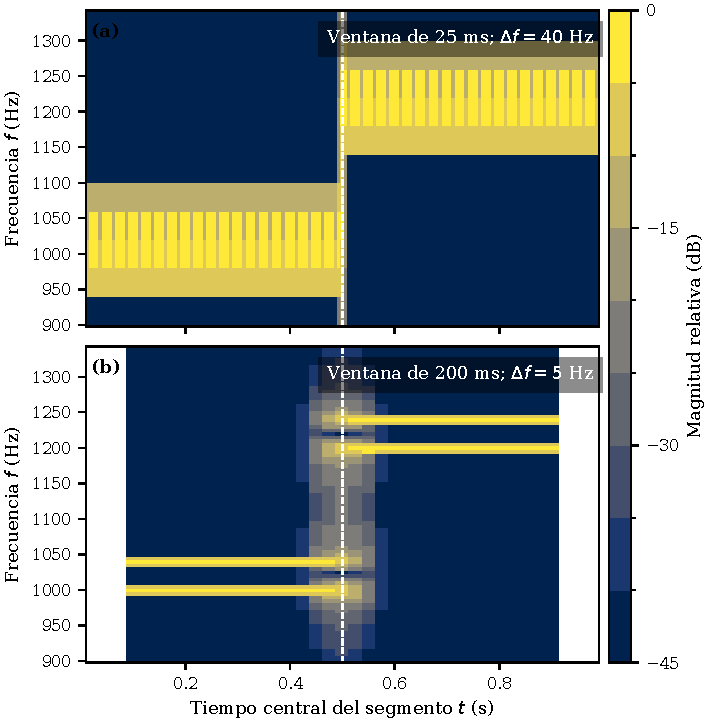
\includegraphics[width=0.96\textwidth]
        {figures/generated/unidad-5/compromiso-tiempo-frecuencia.pdf}
    \caption{Compromiso entre resolución temporal y frecuencial en dos
    espectrogramas de la misma señal teórica, muestreada a
    \(f_s=8000\,\text{Hz}\). Antes de \(0{,}5\,\text{s}\) contiene componentes
    de \(1000\,\text{Hz}\) y \(1040\,\text{Hz}\); después contiene
    \(1200\,\text{Hz}\) y \(1240\,\text{Hz}\). La ventana Hann de
    \(25\,\text{ms}\) produce \(\Delta f=40\,\text{Hz}\); la de
    \(200\,\text{ms}\), \(\Delta f=5\,\text{Hz}\). El color expresa magnitud
    relativa al máximo de cada análisis. Datos sintéticos; elaboración propia.}
    \label{fig:u5-compromiso-tiempo-frecuencia}
\end{figure}

\subsection{Ejemplo resuelto: resolución frecuencial}
\label{sec:u5-ejemplo-resolucion}

Se registra una señal con \(f_s=8000\,\text{Hz}\) y \(N=2000\) muestras.
La duración y la separación entre bins son

\[
    T_\mathrm{obs}=\frac{2000}{8000\,\text{Hz}}
                  =0{,}250\,\text{s},
\]

\[
    \Delta f=\frac{8000\,\text{Hz}}{2000}
            =4{,}0\,\text{Hz}.
\]

Si se mantiene \(f_s=8000\,\text{Hz}\) y se aumenta el registro a
\(N=8000\) muestras, entonces \(T_\mathrm{obs}=1{,}00\,\text{s}\) y
\(\Delta f=1{,}0\,\text{Hz}\). La resolución nominal mejora, aunque ello no
garantiza por sí solo que una estimación sea exacta.

\subsection{Nivel por bin y nivel por banda}
\label{sec:u5-bin-banda}

Un bin representa un intervalo asociado con la resolución del análisis. Si se
modifica \(T_\mathrm{obs}\), cambia \(\Delta f\) y puede cambiar la cantidad
espectral informada en cada bin. Por eso, un ``nivel por bin'' no debe
compararse entre configuraciones sin declarar duración, ventana y
normalización.

Una banda reúne un intervalo de frecuencias definido por un límite inferior
\(f_L\) y uno superior \(f_H\), ambos en hertz. Cuando los valores de los bins
representan contribuciones cuadráticas no correlacionadas \(q_k\), la
contribución de la banda es

\begin{equation}
    q_B=\sum_{k\in B}q_k.
    \label{eq:u5-suma-bins}
\end{equation}

Si cada contribución ya está expresada como un nivel
\(L_k=10\log_{10}(q_k/q_\mathrm{ref})\), el nivel total de la banda se obtiene
mediante

\begin{equation}
    L_B=10\log_{10}
    \left(\sum_{k\in B}10^{L_k/10}\right).
    \label{eq:u5-nivel-banda}
\end{equation}

No corresponde promediar aritméticamente los decibeles. Tampoco deben sumarse
amplitudes sin considerar fase cuando las componentes son coherentes, tal como
se estudió en la Unidad~\ref{chap:unidad-4}.

\section{Espectro de una señal y respuesta de un sistema}
\label{sec:u5-espectro-respuesta}

El \textbf{espectro de una señal} describe la distribución frecuencial de un
registro particular. Si se graba una vocal, el espectro depende de la fuente,
del tracto vocal, de la radiación, del micrófono, del ambiente y del segmento
analizado.

La \textbf{respuesta en frecuencia de un sistema} describe, en cambio, cómo
ese sistema modifica señales de distintas frecuencias. Para un sistema lineal
e invariante en el tiempo, con entrada \(x(t)\), salida \(y(t)\) y
transformadas \(X(f)\) e \(Y(f)\), se define

\begin{equation}
    H(f)=\frac{Y(f)}{X(f)}
    \qquad\text{cuando }X(f)\neq0.
    \label{eq:u5-respuesta-frecuencia}
\end{equation}

La magnitud \(\lvert H(f)\rvert\) informa el cambio de amplitud y la fase
\(\phi_H(f)\), en radianes, informa el cambio de fase. Si entrada y salida
representan la misma magnitud física, el cociente es adimensional y su
ganancia de amplitud puede expresarse como

\begin{equation}
    G(f)=20\log_{10}\lvert H(f)\rvert,
    \label{eq:u5-ganancia-respuesta}
\end{equation}

donde \(G(f)\) se expresa en decibeles. Una respuesta no puede deducirse de la
salida solamente: se necesita conocer la entrada o emplear un procedimiento
de medición equivalente.

La figura~\ref{fig:u5-espectro-respuesta-sistema} compara las tres cantidades
con una escala común. Los paneles de entrada y salida son espectros de señales;
el panel central es una propiedad del sistema dentro del modelo lineal.

\begin{figure}[htbp]
    \centering
    % Propósito: distinguir los espectros de entrada y salida de la respuesta en
% frecuencia del sistema que los relaciona.
% Origen: Y(f)=X(f)H(f). Se usan magnitudes normalizadas y datos teóricos:
% |X|=(0,8;0,8;0,8), |H|=(1;0,5;0,25) para f=(0,5;1;2) kHz;
% por lo tanto |Y|=(0,8;0,4;0,2).
% Esquema matemático; no representa un dispositivo ni una medición real.
% Descripción accesible: tres paneles muestran, de izquierda a derecha, un
% espectro de entrada con tres componentes iguales, una respuesta de sistema
% que atenúa progresivamente esas frecuencias y un espectro de salida cuyos
% componentes son los productos de entrada y respuesta. La figura enfatiza que
% el espectro pertenece a una señal y H pertenece al sistema.
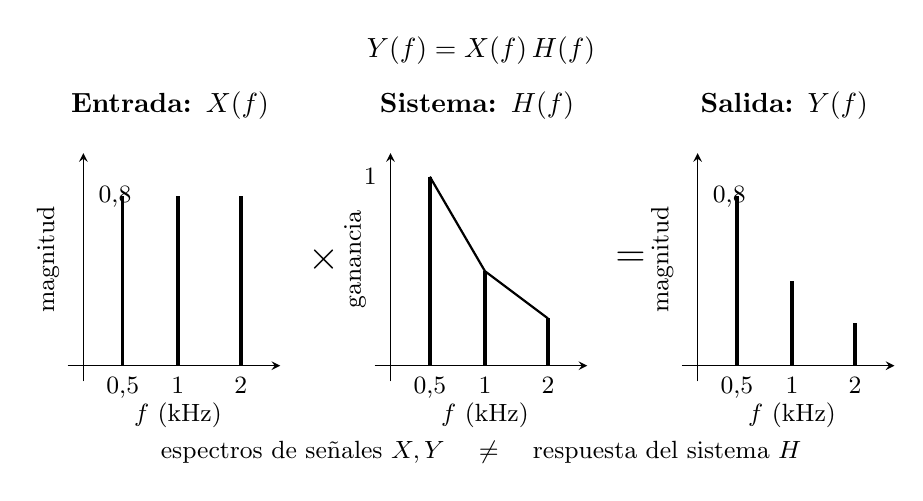
\begin{tikzpicture}[font=\small,>=stealth,x=1cm,y=1cm]
    \node[font=\bfseries] at (5.75,4.75)
        {\(\lvert Y(f)\rvert=\lvert X(f)\rvert\,\lvert H(f)\rvert\)};

    \begin{scope}[shift={(0.15,0)}]
        \node[font=\bfseries] at (1.65,4.05) {Entrada: \(\lvert X(f)\rvert\)};
        \draw[->] (0.35,0.75) -- (3.05,0.75);
        \draw[->] (0.55,0.55) -- (0.55,3.45);
        \node[rotate=90] at (0.10,2.10) {magnitud};
        \draw[very thick] (1.05,0.75) -- (1.05,2.90);
        \draw[very thick] (1.75,0.75) -- (1.75,2.90);
        \draw[very thick] (2.55,0.75) -- (2.55,2.90);
        \foreach \x/\lab in {1.05/0{,}5,1.75/1,2.55/2}
            \node[below] at (\x,0.72) {\lab};
        \node[anchor=west] at (0.62,2.90) {\(0{,}8\)};
        \node at (1.75,0.12) {\(f\) (kHz)};
    \end{scope}

    \node[font=\Large] at (3.75,2.10) {\(\times\)};

    \begin{scope}[shift={(4.05,0)}]
        \node[font=\bfseries] at (1.65,4.05) {Sistema: \(\lvert H(f)\rvert\)};
        \draw[->] (0.35,0.75) -- (3.05,0.75);
        \draw[->] (0.55,0.55) -- (0.55,3.45);
        \node[rotate=90] at (0.10,2.10) {ganancia};
        \draw[very thick] (1.05,0.75) -- (1.05,3.15);
        \draw[very thick] (1.75,0.75) -- (1.75,1.95);
        \draw[very thick] (2.55,0.75) -- (2.55,1.35);
        \draw[thick] (1.05,3.15) -- (1.75,1.95) -- (2.55,1.35);
        \foreach \x/\lab in {1.05/0{,}5,1.75/1,2.55/2}
            \node[below] at (\x,0.72) {\lab};
        \node[anchor=east] at (0.50,3.15) {\(1\)};
        \node at (1.75,0.12) {\(f\) (kHz)};
    \end{scope}

    \node[font=\Large] at (7.65,2.10) {\(=\)};

    \begin{scope}[shift={(7.95,0)}]
        \node[font=\bfseries] at (1.65,4.05) {Salida: \(\lvert Y(f)\rvert\)};
        \draw[->] (0.35,0.75) -- (3.05,0.75);
        \draw[->] (0.55,0.55) -- (0.55,3.45);
        \node[rotate=90] at (0.10,2.10) {magnitud};
        \draw[very thick] (1.05,0.75) -- (1.05,2.90);
        \draw[very thick] (1.75,0.75) -- (1.75,1.83);
        \draw[very thick] (2.55,0.75) -- (2.55,1.29);
        \foreach \x/\lab in {1.05/0{,}5,1.75/1,2.55/2}
            \node[below] at (\x,0.72) {\lab};
        \node[anchor=west] at (0.62,2.90) {\(0{,}8\)};
        \node at (1.75,0.12) {\(f\) (kHz)};
    \end{scope}

    \node[align=center] at (5.75,-0.35)
        {espectros de señales \(\lvert X\rvert,\lvert Y\rvert\)
         \(\quad\neq\quad\) respuesta del sistema \(\lvert H\rvert\)};
\end{tikzpicture}

    \caption{Relación entre los espectros de magnitud de entrada y salida y la
    magnitud de la respuesta de un sistema. En este ejemplo teórico,
    \(\lvert Y(f)\rvert=\lvert X(f)\rvert\lvert H(f)\rvert\) en tres
    frecuencias. Conocer solo \(\lvert Y(f)\rvert\) no permite separar cuánto
    corresponde a la señal de entrada y cuánto al sistema. Magnitudes
    normalizadas; elaboración propia.}
    \label{fig:u5-espectro-respuesta-sistema}
\end{figure}

Si un sistema introduce únicamente un retraso \(\tau\), medido en segundos,
la magnitud de su respuesta ideal permanece igual a uno y el cambio de fase es

\begin{equation}
    \phi_H(f)=-2\pi f\tau,
    \label{eq:u5-fase-retardo}
\end{equation}

donde \(\phi_H(f)\) se expresa en radianes. Este ejemplo muestra que una
respuesta puede modificar la fase sin modificar la magnitud.

En producción vocal, una descripción introductoria considera una fuente
glótica y un tracto vocal que actúa como sistema acústico. Los formantes se
relacionan con resonancias del tracto y suelen observarse en la envolvente
espectral, mientras que las líneas armónicas se relacionan con la periodicidad
de la fuente. La interpretación de formantes y otros parámetros de voz
requiere definir la vocal, el hablante, el método de análisis y el alcance
clínico, además de incorporar bibliografía especializada~\cite{brockmann2011}.

\subsection{Ejemplo resuelto: ganancia a una frecuencia}
\label{sec:u5-ejemplo-respuesta}

Un sistema recibe un tono de \(1000\,\text{Hz}\) con presión eficaz de entrada
\(p_\mathrm{in}=0{,}020\,\text{Pa}\) y produce una presión eficaz de salida
\(p_\mathrm{out}=0{,}010\,\text{Pa}\), medidas bajo las mismas condiciones.
La magnitud de la respuesta a esa frecuencia es

\[
    \lvert H(1000\,\text{Hz})\rvert
    =\frac{0{,}010\,\text{Pa}}{0{,}020\,\text{Pa}}
    =0{,}50.
\]

La ganancia es

\[
    G(1000\,\text{Hz})
    =20\log_{10}(0{,}50)
    \approx-6{,}02\,\text{dB}.
\]

El resultado indica una reducción de amplitud a \(1000\,\text{Hz}\). No
describe el espectro completo de la entrada ni permite conocer la respuesta
del sistema en otras frecuencias.

\section{Componentes espectrales}
\label{sec:u5-componentes}

\begin{description}[style=nextline]
    \item[\textbf{Frecuencia fundamental (\(f_0\)):}]
    inversa del período fundamental \(T_0\) de una señal periódica. No tiene
    que coincidir con la componente de mayor amplitud.

    \item[\textbf{Armónico:}]
    componente cuya frecuencia es \(nf_0\), donde \(n\) es un entero
    positivo. El primer armónico corresponde a \(f_0\), si esa componente está
    presente.

    \item[\textbf{Parcial:}]
    componente sinusoidal identificable en una señal compleja. Los parciales
    pueden ser armónicos o inarmónicos.

    \item[\textbf{Sobretono:}]
    parcial situado por encima de la fundamental en el uso musical y
    acústico habitual. El primer sobretono es el segundo parcial, por lo que
    no debe confundirse con el primer armónico.

    \item[\textbf{Parcial inarmónico:}]
    componente cuya frecuencia no coincide con un múltiplo entero de
    \(f_0\).
\end{description}

Una señal periódica puede conservar su periodicidad aunque la línea en
\(f_0\) tenga amplitud nula. En ese caso se habla de una fundamental ausente:
las separaciones entre armónicos todavía pueden revelar la periodicidad. El
\emph{pitch} asociado con este tipo de estímulos es un fenómeno perceptual y
se desarrollará en el capítulo dedicado a psicoacústica; no se identifica con
una línea espectral por definición.

La figura~\ref{fig:u5-componentes-espectrales} reúne tres casos con igual
escala. Permite comprobar que el componente de mayor amplitud no define
\(f_0\), que no todo parcial es armónico y que una periodicidad puede
manifestarse por la separación entre líneas aun si falta la componente
fundamental.

\begin{figure}[htbp]
    \centering
    % Propósito: diferenciar armónicos, parciales, sobretonos, componente de mayor
% amplitud y fundamental ausente mediante espectros con una misma escala.
% Origen: datos teóricos de magnitud normalizada. Panel armónico:
% f=(100,200,300,400) Hz y A=(0,45;1;0,60;0,30). Panel inarmónico:
% f=(100,235,370,520) Hz y A=(0,60;1;0,55;0,30). Fundamental ausente:
% f=(200,300,400) Hz y A=(1;0,60;0,40), con separación de 100 Hz.
% No representa sonidos medidos ni instrumentos particulares.
% Descripción accesible: el primer panel tiene líneas en múltiplos de 100 Hz y
% muestra que el segundo armónico puede superar a la fundamental. El segundo
% presenta parciales que no son múltiplos enteros. El tercero omite la línea de
% 100 Hz, pero conserva líneas separadas 100 Hz, de modo que la periodicidad
% fundamental puede inferirse aunque esa componente esté ausente.
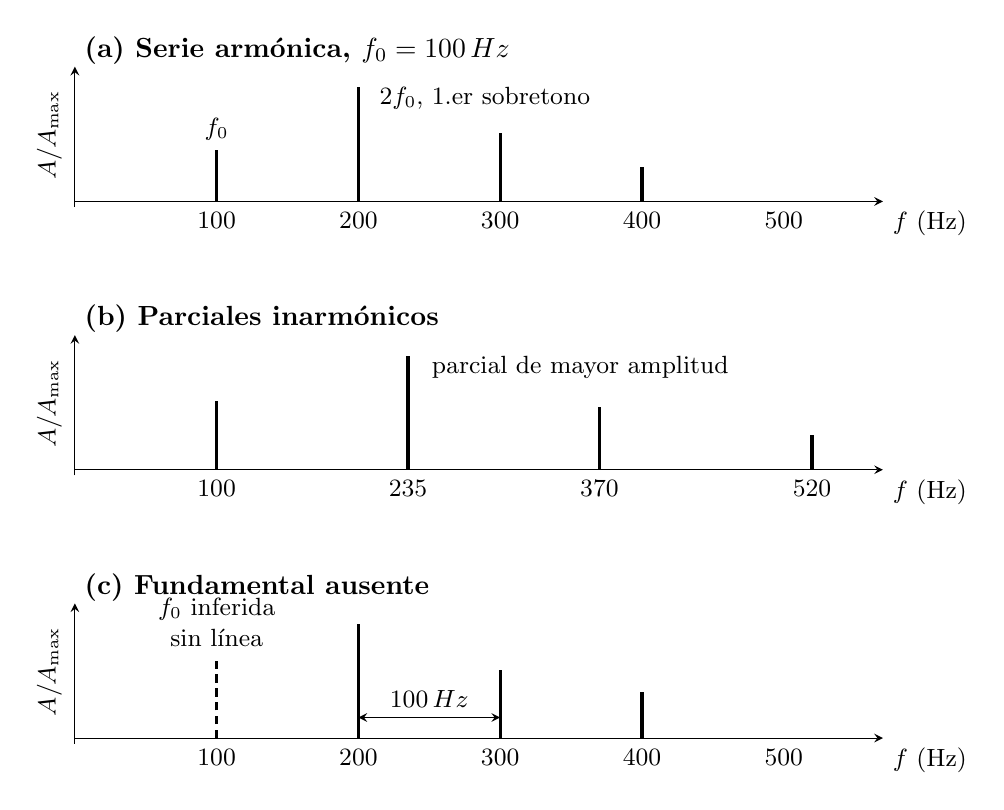
\begin{tikzpicture}[font=\small,>=stealth,x=0.018cm,y=1.45cm]
    \begin{scope}[shift={(0,4.55)}]
        \node[anchor=west,font=\bfseries] at (0,1.32)
            {(a) Serie armónica, \(f_0=100\,\text{Hz}\)};
        \draw[->] (0,0) -- (570,0) node[below right] {\(f\) (Hz)};
        \draw[->] (0,-0.05) -- (0,1.18);
        \node[rotate=90] at (-18,0.58) {\(A/A_{\max}\)};
        \foreach \f/\a in {100/0.45,200/1.00,300/0.60,400/0.30}
            \draw[very thick] (\f,0) -- (\f,\a);
        \foreach \f in {100,200,300,400,500}
            \node[below] at (\f,-0.01) {\f};
        \node[above,align=center] at (100,0.45) {\(f_0\)};
        \node[anchor=west,align=left] at (208,0.90)
            {\(2f_0\), 1.er sobretono};
    \end{scope}

    \begin{scope}[shift={(0,2.20)}]
        \node[anchor=west,font=\bfseries] at (0,1.32)
            {(b) Parciales inarmónicos};
        \draw[->] (0,0) -- (570,0) node[below right] {\(f\) (Hz)};
        \draw[->] (0,-0.05) -- (0,1.18);
        \node[rotate=90] at (-18,0.58) {\(A/A_{\max}\)};
        \foreach \f/\a in {100/0.60,235/1.00,370/0.55,520/0.30}
            \draw[very thick] (\f,0) -- (\f,\a);
        \foreach \f in {100,235,370,520}
            \node[below] at (\f,-0.01) {\f};
        \node[anchor=west] at (245,0.90) {parcial de mayor amplitud};
    \end{scope}

    \begin{scope}[shift={(0,-0.15)}]
        \node[anchor=west,font=\bfseries] at (0,1.32)
            {(c) Fundamental ausente};
        \draw[->] (0,0) -- (570,0) node[below right] {\(f\) (Hz)};
        \draw[->] (0,-0.05) -- (0,1.18);
        \node[rotate=90] at (-18,0.58) {\(A/A_{\max}\)};
        \draw[very thick,densely dashed] (100,0) -- (100,0.72);
        \foreach \f/\a in {200/1.00,300/0.60,400/0.40}
            \draw[very thick] (\f,0) -- (\f,\a);
        \foreach \f in {100,200,300,400,500}
            \node[below] at (\f,-0.01) {\f};
        \node[above,align=center] at (100,0.72)
            {\(f_0\) inferida\\sin línea};
        \draw[<->] (200,0.18) -- (300,0.18)
            node[midway,above] {\(100\,\text{Hz}\)};
    \end{scope}
\end{tikzpicture}

    \caption{Comparación de espectros de líneas teóricos con magnitud
    normalizada. (a)~Serie armónica de \(f_0=100\,\text{Hz}\), cuyo segundo
    armónico posee la mayor amplitud; el primer sobretono coincide aquí con el
    segundo armónico. (b)~Parciales inarmónicos, que no siguen múltiplos
    enteros. (c)~Fundamental ausente: no aparece una línea en
    \(100\,\text{Hz}\), pero las componentes conservan esa separación.
    Elaboración propia; no son registros de fuentes reales.}
    \label{fig:u5-componentes-espectrales}
\end{figure}

\section{Rangos de frecuencia y rangos dinámicos}
\label{sec:u5-rangos}

\subsection{Infrasonido, rango audible y ultrasonido}
\label{sec:u5-infra-audible-ultra}

Se usa de manera convencional \(20\,\text{Hz}\) como frontera entre
infrasonido y rango audible, y \(20\,\text{kHz}\) como frontera entre rango
audible y ultrasonido; estos límites son aproximados y requieren una fuente
académica que declare las condiciones de escucha~\cite{oxenham2018,iso226_2023}.

El término \textbf{infrasonido} describe frecuencias inferiores a la frontera
convencional de \(20\,\text{Hz}\). No significa que toda señal de esa región
sea necesariamente imperceptible: la detección puede depender del
nivel, la duración, la distorsión del sistema y la presencia de vibración~\cite{oxenham2018,iso226_2023}.

El \textbf{rango audible} no es idéntico para todas las personas ni para todos
los niveles. La sensibilidad varía con la frecuencia y con características
del oyente. Estas dependencias perceptuales se estudiarán posteriormente.

El \textbf{ultrasonido} corresponde a frecuencias superiores a la frontera
convencional de \(20\,\text{kHz}\). Una aplicación médica general es la
formación de imágenes mediante ultrasonido; las otoemisiones acústicas no
deben presentarse como ejemplo de ultrasonido sin especificar las frecuencias
de estímulo y registro.

\subsection{Qué significa rango dinámico}
\label{sec:u5-rango-dinamico}

El \textbf{rango dinámico} compara un nivel superior y uno inferior que deben
estar definidos mediante la misma magnitud, referencia y condición de
medición. Si \(L_\mathrm{sup}\) y \(L_\mathrm{inf}\) son esos niveles, el
rango dinámico es

\begin{equation}
    R_D=L_\mathrm{sup}-L_\mathrm{inf},
    \label{eq:u5-rango-dinamico}
\end{equation}

y se expresa en decibeles. La resta informa una relación; no debe interpretarse
sin conocer cómo se eligieron los extremos.

\begin{description}[style=nextline]
    \item[\textbf{Rango dinámico vocal:}]
    diferencia entre niveles relevantes de una producción vocal bajo una
    condición declarada. Deben especificarse distancia, dirección,
    ponderación, descriptor temporal y tarea de emisión.

    \item[\textbf{Rango dinámico instrumental:}]
    diferencia entre niveles relevantes producidos por un instrumento bajo
    condiciones definidas. No es un valor universal del instrumento: depende
    de técnica, nota, sala y posición de medición.

    \item[\textbf{Rango dinámico auditivo:}]
    intervalo entre un límite inferior de audibilidad y un límite superior
    definido, por ejemplo un nivel de incomodidad, para una frecuencia,
    estímulo y oyente determinados. No corresponde reemplazar automáticamente
    el límite superior por un ``umbral de dolor'' universal.
\end{description}

Los valores numéricos de rangos vocales, instrumentales y auditivos
deben incorporarse solo después de seleccionar fuentes, condiciones de
medición y población de referencia~\cite{oxenham2018,iso226_2023}.

\section{Bandas de octava y tercio de octava}
\label{sec:u5-bandas}

Agrupar frecuencias en bandas permite resumir un espectro con una resolución
relativa aproximadamente constante. Una banda se define mediante su límite
inferior \(f_L\), su límite superior \(f_H\) y su frecuencia central
geométrica \(f_c\), todas medidas en hertz:

\begin{equation}
    f_c=\sqrt{f_Lf_H}.
    \label{eq:u5-centro-geometrico}
\end{equation}

Para una fracción \(1/b\) de octava, la razón entre límites es

\begin{equation}
    \frac{f_H}{f_L}=2^{1/b}.
    \label{eq:u5-razon-banda}
\end{equation}

Los límites alrededor de \(f_c\) son

\begin{equation}
    f_L=f_c\,2^{-1/(2b)},
    \qquad
    f_H=f_c\,2^{1/(2b)}.
    \label{eq:u5-limites-banda}
\end{equation}

El ancho de banda \(B\), medido en hertz, se define como

\begin{equation}
    B=f_H-f_L.
    \label{eq:u5-ancho-banda}
\end{equation}

Para una octava, \(b=1\) y \(f_H/f_L=2\). Para un tercio de octava,
\(b=3\) y \(f_H/f_L=2^{1/3}\). Los instrumentos normalizados usan
series de frecuencias centrales nominales y requisitos de tolerancia que deben
documentarse con la edición aplicable de la norma de filtros de banda~\cite{iec61260_1_2014}.

\subsection{Ejemplo resuelto: tercio de octava}
\label{sec:u5-ejemplo-tercio}

Para \(f_c=1000\,\text{Hz}\) y \(b=3\):

\[
    f_L=1000\,\text{Hz}\,2^{-1/6}
       \approx890{,}9\,\text{Hz},
\]

\[
    f_H=1000\,\text{Hz}\,2^{1/6}
       \approx1122{,}5\,\text{Hz}.
\]

Por lo tanto,

\[
    B\approx1122{,}5\,\text{Hz}-890{,}9\,\text{Hz}
      \approx231{,}6\,\text{Hz}.
\]

Los valores redondeados \(891\,\text{Hz}\) y \(1122\,\text{Hz}\) son límites
aproximados; el ancho no es \(176\,\text{Hz}\).

La división completa se muestra en la
figura~\ref{fig:u5-bandas-octava-tercio}. Sobre el eje logarítmico, los tres
tercios ocupan igual longitud porque comparten la misma razón entre límites;
sus anchos absolutos en hertz, en cambio, no son iguales.

\begin{figure}[htbp]
    \centering
    % Propósito: mostrar que una octava puede dividirse en tres tercios contiguos
% sobre un eje logarítmico y que el ancho absoluto crece con la frecuencia.
% Origen: ecuaciones f_L=f_c 2^{-1/(2b)}, f_H=f_c 2^{1/(2b)} y B=f_H-f_L.
% Para la octava centrada en 1000 Hz: límites 707,1 y 1414,2 Hz.
% Los tres tercios tienen centros 793,7; 1000 y 1259,9 Hz, límites comunes
% 707,1; 890,9; 1122,5; 1414,2 Hz y anchos 183,8; 231,6; 291,8 Hz.
% Esquema matemático sobre eje logarítmico; no representa filtros medidos.
% Descripción accesible: una barra superior abarca la octava de 707,1 a
% 1414,2 Hz alrededor de 1000 Hz. Debajo, tres barras contiguas ocupan el mismo
% intervalo sobre el eje logarítmico. Aunque tienen la misma razón entre
% límites, sus anchos en hertz aumentan hacia frecuencias más altas.
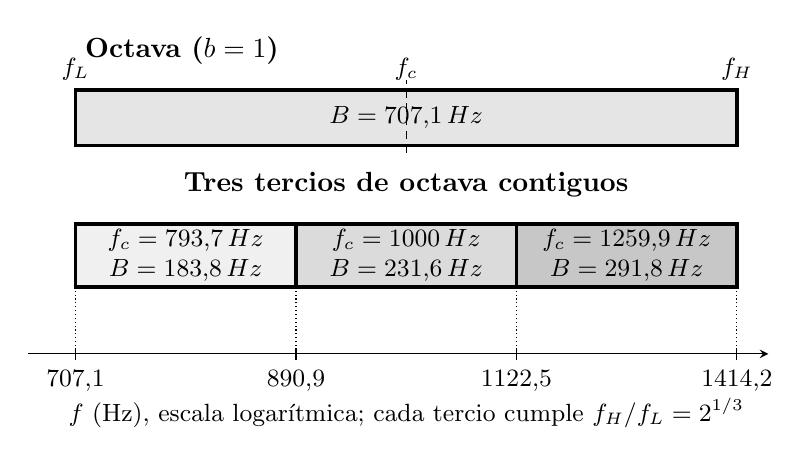
\begin{tikzpicture}[font=\small,>=stealth,x=1cm,y=1cm]
    \node[anchor=west,font=\bfseries] at (1.40,4.55)
        {Octava (\(b=1\))};

    \draw[fill=black!10] (1.40,3.35) rectangle (9.80,4.05);
    \draw[very thick] (1.40,3.35) rectangle (9.80,4.05);
    \draw[densely dashed] (5.60,3.25) -- (5.60,4.18);
    \node at (5.60,3.70) {\(B=707{,}1\,\text{Hz}\)};
    \node[above] at (1.40,4.05) {\(f_L\)};
    \node[above] at (5.60,4.05) {\(f_c\)};
    \node[above] at (9.80,4.05) {\(f_H\)};

    \node[font=\bfseries] at (5.60,2.85)
        {Tres tercios de octava contiguos};
    \draw[fill=black!6] (1.40,1.55) rectangle (4.20,2.35);
    \draw[fill=black!14] (4.20,1.55) rectangle (7.00,2.35);
    \draw[fill=black!22] (7.00,1.55) rectangle (9.80,2.35);
    \draw[very thick] (1.40,1.55) rectangle (9.80,2.35);
    \draw[very thick] (4.20,1.55) -- (4.20,2.35);
    \draw[very thick] (7.00,1.55) -- (7.00,2.35);
    \node[align=center] at (2.80,1.95)
        {\(f_c=793{,}7\,\text{Hz}\)\\\(B=183{,}8\,\text{Hz}\)};
    \node[align=center] at (5.60,1.95)
        {\(f_c=1000\,\text{Hz}\)\\\(B=231{,}6\,\text{Hz}\)};
    \node[align=center] at (8.40,1.95)
        {\(f_c=1259{,}9\,\text{Hz}\)\\\(B=291{,}8\,\text{Hz}\)};

    \draw[->] (0.80,0.70) -- (10.20,0.70);
    \foreach \x/\lab in {
        1.40/707{,}1,
        4.20/890{,}9,
        7.00/1122{,}5,
        9.80/1414{,}2
    }{
        \draw (\x,0.62) -- (\x,0.78);
        \node[below] at (\x,0.62) {\lab};
        \draw[densely dotted] (\x,0.80) -- (\x,1.50);
    }
    \node[align=center] at (5.60,-0.05)
        {\(f\) (Hz), escala logarítmica;
         cada tercio cumple \(f_H/f_L=2^{1/3}\)};
\end{tikzpicture}

    \caption{Una octava centrada en \(1000\,\text{Hz}\) y su división en tres
    tercios contiguos. Los límites se calcularon con
    \(f_L=f_c2^{-1/(2b)}\) y \(f_H=f_c2^{1/(2b)}\). Las bandas tienen el mismo
    ancho relativo sobre el eje logarítmico, pero \(B=f_H-f_L\) aumenta con la
    frecuencia. Valores teóricos redondeados a \(0{,}1\,\text{Hz}\);
    elaboración propia.}
    \label{fig:u5-bandas-octava-tercio}
\end{figure}

\section{Filtros y respuesta en frecuencia}
\label{sec:u5-filtros}

Un filtro es un sistema que modifica componentes de una señal según la
frecuencia. Un filtro \textbf{ideal} cambia abruptamente entre paso y rechazo.
Un filtro \textbf{real} posee regiones de transición, atenuación finita y una
respuesta de fase que puede modificar la forma temporal.

\begin{description}[style=nextline]
    \item[\textbf{Pasa bajos:}]
    conserva una banda de bajas frecuencias y atenúa frecuencias por encima de
    su transición.

    \item[\textbf{Pasa altos:}]
    conserva una banda de altas frecuencias y atenúa frecuencias por debajo de
    su transición.

    \item[\textbf{Pasa banda:}]
    conserva un intervalo entre un límite inferior \(f_L\) y uno superior
    \(f_H\).

    \item[\textbf{Elimina banda o rechazo de banda:}]
    atenúa un intervalo entre \(f_L\) y \(f_H\) y conserva frecuencias por
    debajo y por encima. Un filtro \emph{notch} es un rechazo relativamente
    estrecho.
\end{description}

La \textbf{frecuencia de corte} debe asociarse con un criterio de atenuación
declarado. En modelos comunes se usa el punto de \(-3\,\text{dB}\), pero esa
convención no es universal para todo filtro o instrumento. En filtros pasa
banda y elimina banda se requieren, como mínimo, dos frecuencias límite. Su
frecuencia central puede definirse geométricamente como

\[
    f_c=\sqrt{f_Lf_H},
\]

y su ancho como \(B=f_H-f_L\), ambos con las mismas definiciones y unidades
empleadas para las bandas.

La figura~\ref{fig:u5-filtros-ideales-reales} compara el salto matemático ideal
con modelos no ideales que poseen transición. Las líneas verticales sirven para
ubicar \(f_c\), \(f_L\) y \(f_H\); no deben interpretarse como especificaciones
de un instrumento particular.

\begin{figure}[htbp]
    \centering
    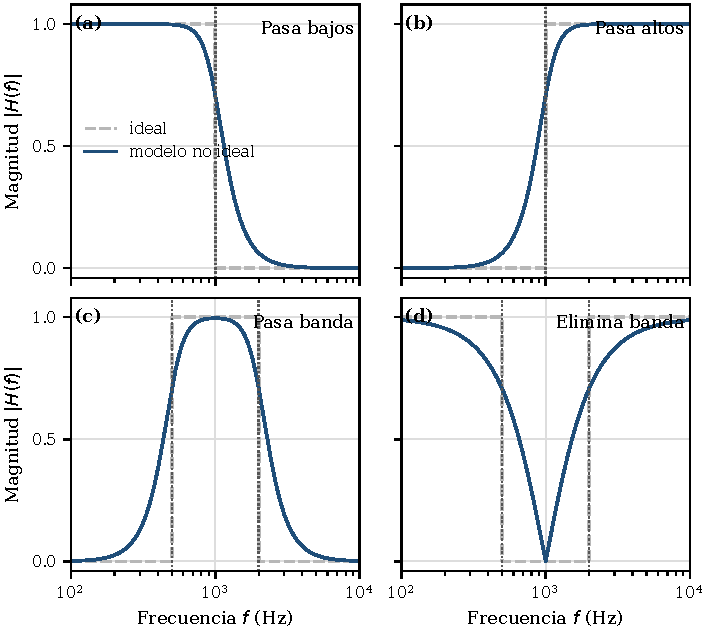
\includegraphics[width=0.96\textwidth]
        {figures/generated/unidad-5/filtros-ideales-reales.pdf}
    \caption{Respuestas de magnitud ideales y modelos analíticos no ideales para
    filtros pasa bajos, pasa altos, pasa banda y elimina banda. Los pasa bajos y
    pasa altos usan modelos Butterworth de cuarto orden con
    \(f_c=1000\,\text{Hz}\); el pasa banda combina límites de
    \(f_L=500\,\text{Hz}\) y \(f_H=2000\,\text{Hz}\), y el rechazo usa un
    modelo de segundo orden con \(f_c=\sqrt{f_Lf_H}=1000\,\text{Hz}\).
    Curvas teóricas, no respuestas medidas; elaboración propia.}
    \label{fig:u5-filtros-ideales-reales}
\end{figure}

\subsection{Filtrado, ponderación y filtrado audiométrico}
\label{sec:u5-filtros-ponderacion-audiometria}

Estas operaciones pueden usar filtros, pero no tienen el mismo propósito:

\begin{description}[style=nextline]
    \item[\textbf{Filtrado de una señal:}]
    modifica el contenido espectral de la señal que se procesa o reproduce.

    \item[\textbf{Ponderación frecuencial de una medición:}]
    aplica una respuesta estandarizada antes de calcular e informar un nivel.
    La ponderación debe aparecer en el símbolo o en la unidad informada.

    \item[\textbf{Filtrado audiométrico:}]
    forma parte de la generación o control de estímulos de un audiómetro, por
    ejemplo al delimitar una banda de ruido. Sus requisitos dependen del
    equipo, del estímulo y de la calibración audiométrica.
\end{description}

Una ponderación A no convierte un nivel en dB SPL a dB HL. El nivel de audición
en dB HL depende de frecuencia, transductor y referencias de calibración
específicas.

\section{Ponderaciones frecuenciales A, C y Z}
\label{sec:u5-ponderaciones}

Una ponderación frecuencial es una respuesta de medición definida en función
de la frecuencia. Si \(L_Z(f)\) es el nivel de un tono medido con ponderación
Z y \(A(f)\) es la corrección de la ponderación A a esa frecuencia, expresada
en decibeles, entonces, bajo las mismas condiciones,

\begin{equation}
    L_A(f)=L_Z(f)+A(f).
    \label{eq:u5-correccion-ponderacion}
\end{equation}

La ponderación A atenúa con fuerza las bajas frecuencias y modifica también la
respuesta en otras regiones. La ponderación C posee una respuesta más plana
en una región amplia, pero tampoco es una medición sin filtro. La ponderación
Z es una respuesta nominalmente plana dentro de un intervalo y unas
tolerancias especificadas; no representa ``el sonido real'' sin límites.

Las respuestas nominales, los límites de aceptación, el intervalo de
frecuencias y las denominaciones de A, C y Z se especifican en la edición
aplicable de la norma de sonómetros~\cite{iec61672_1_2013}.

Para una señal de banda ancha no corresponde tomar un nivel total y agregar
una única corrección elegida de una tabla. La ponderación actúa de manera
diferente en cada frecuencia; el instrumento filtra la señal y luego realiza
la integración energética.

\subsection{Ejemplo resuelto: corrección para un tono}
\label{sec:u5-ejemplo-ponderacion}

La tabla 3 de IEC 61672-1:2013 establece, como valor nominal de la
ponderación A a \(63\,\text{Hz}\),
\(A(63\,\text{Hz})=-26{,}2\,\text{dB}\)~\cite{iec61672_1_2013}. Si un tono de
\(63\,\text{Hz}\) produce \(L_Z=80{,}0\,\text{dB(Z)}\), entonces

\[
    L_A=80{,}0\,\text{dB(Z)}-26{,}2\,\text{dB}
       =53{,}8\,\text{dB(A)}.
\]

El cálculo se aplica a ese tono y a la corrección proporcionada. No implica
que cualquier sonido de \(80\,\text{dB(Z)}\) produzca
\(53{,}8\,\text{dB(A)}\).

% TODO(figure): evaluar una figura original de las curvas nominales A, C y Z
% calculadas con las expresiones del anexo E de IEC 61672-1:2013; diferenciar
% esas curvas de los límites de aceptación de un instrumento.

\section{Sonómetro}
\label{sec:u5-sonometro}

Un sonómetro recibe una señal de micrófono y la procesa para informar niveles
acústicos definidos. Una cadena funcional básica incluye:

\begin{enumerate}
    \item \textbf{micrófono:} convierte la presión acústica local, en
    pascales, en una señal eléctrica. Un micrófono con corrección de campo
    libre no elimina las reflexiones del ambiente;
    \item \textbf{preamplificación y conversión:} adapta y, en instrumentos
    digitales, muestrea la señal;
    \item \textbf{ponderación frecuencial:} aplica A, C, Z u otra respuesta
    disponible y declarada;
    \item \textbf{detector o integrador:} calcula una medida cuadrática,
    temporal o de exposición;
    \item \textbf{ponderación temporal:} determina cómo responde la indicación
    ante cambios rápidos;
    \item \textbf{visualización y almacenamiento:} informa la magnitud, la
    ponderación, el intervalo temporal y, cuando corresponda, incertidumbre o
    estado del instrumento.
\end{enumerate}

La figura~\ref{fig:u5-cadena-sonometro} resume el recorrido de la información.
La presión acústica existe antes de la medición; el valor informado aparece
después de las conversiones, ponderaciones e integraciones elegidas.

\begin{figure}[htbp]
    \centering
    % Propósito: seguir la transformación desde una presión acústica local hasta
% un nivel informado por un sonómetro y distinguir señal física, procesamiento
% y resultado.
% Origen: cadena funcional conceptual descrita en la sección Sonómetro de la
% Unidad 5. No representa la arquitectura interna de un modelo comercial ni
% especifica requisitos normativos.
% Descripción accesible: seis bloques conectados muestran micrófono,
% preamplificación y conversión, ponderación frecuencial, detector o integrador,
% ponderación temporal, y visualización y almacenamiento. La entrada es presión
% acústica en pascales; la salida es un nivel acompañado por su ponderación e
% intervalo temporal.
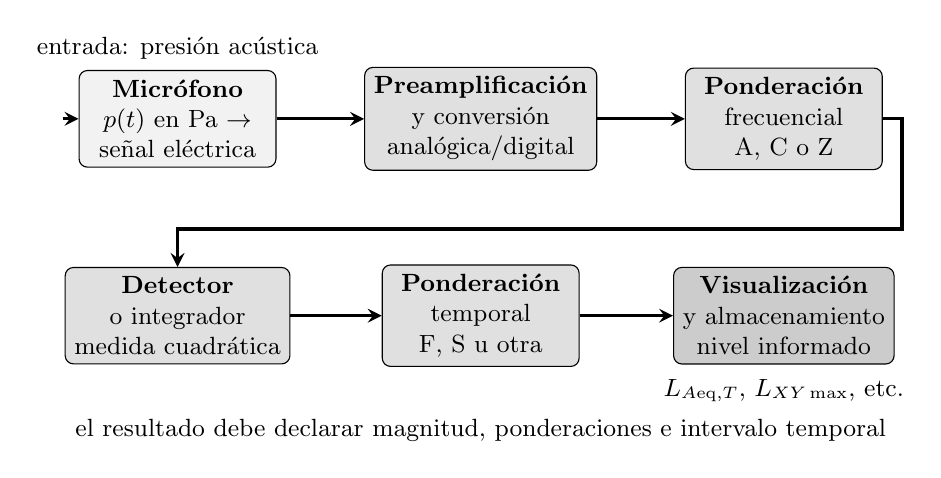
\begin{tikzpicture}[font=\small,>=stealth,x=1cm,y=1cm]
    \tikzset{
        block/.style={
            draw,
            rounded corners=3pt,
            minimum width=2.50cm,
            minimum height=1.10cm,
            align=center
        },
        signal/.style={block,fill=black!5},
        process/.style={block,fill=black!12},
        result/.style={block,fill=black!20}
    }

    \node[signal] (mic) at (1.45,3.15)
        {\textbf{Micrófono}\\
         \(p(t)\) en Pa \(\rightarrow\)\\señal eléctrica};
    \node[process] (pre) at (5.30,3.15)
        {\textbf{Preamplificación}\\
         y conversión\\analógica/digital};
    \node[process] (freq) at (9.15,3.15)
        {\textbf{Ponderación}\\
         frecuencial\\A, C o Z};

    \node[process] (det) at (1.45,0.65)
        {\textbf{Detector}\\
         o integrador\\medida cuadrática};
    \node[process] (time) at (5.30,0.65)
        {\textbf{Ponderación}\\
         temporal\\F, S u otra};
    \node[result] (display) at (9.15,0.65)
        {\textbf{Visualización}\\
         y almacenamiento\\nivel informado};

    \node at (1.45,4.05) {entrada: presión acústica};
    \draw[->,very thick] (0.00,3.15) -- (mic.west);
    \draw[->,very thick] (mic.east) -- (pre.west);
    \draw[->,very thick] (pre.east) -- (freq.west);
    \draw[->,very thick] (freq.east) -- (10.65,3.15)
        -- (10.65,1.75) -- (1.45,1.75) -- (det.north);
    \draw[->,very thick] (det.east) -- (time.west);
    \draw[->,very thick] (time.east) -- (display.west);
    \node[align=center] at (9.15,-0.30)
        {\(L_{A\mathrm{eq},T}\), \(L_{XY\max}\), etc.};

    \node[align=center] at (5.30,-0.80)
        {el resultado debe declarar magnitud, ponderaciones e intervalo temporal};
\end{tikzpicture}

    \caption{Cadena funcional introductoria de un sonómetro. El micrófono
    convierte la presión acústica local \(p(t)\), en pascales, en una señal
    eléctrica; los bloques posteriores la acondicionan y procesan hasta obtener
    un nivel con ponderaciones e intervalo declarados. El diagrama es
    conceptual y no representa la arquitectura interna de un modelo comercial
    ni sustituye requisitos normativos. Elaboración propia.}
    \label{fig:u5-cadena-sonometro}
\end{figure}

\subsection{Nivel equivalente}
\label{sec:u5-leq}

Sea \(p_X(t)\) la presión acústica después de aplicar una ponderación
frecuencial \(X\), medida en pascales, durante un intervalo \(T\), medido en
segundos. La letra \(X\) identifica la ponderación frecuencial, por ejemplo A,
C o Z. El nivel equivalente es

\begin{equation}
    L_{X\mathrm{eq},T}
    =10\log_{10}
    \left[
        \frac{1}{T}
        \int_0^T
        \frac{p_X^2(t)}{p_\mathrm{ref}^{\,2}}\,dt
    \right],
    \label{eq:u5-leq}
\end{equation}

donde \(p_\mathrm{ref}=20\,\mu\text{Pa}\) en aire para nivel de presión
sonora. Si se usa ponderación A, se escribe \(L_{A\mathrm{eq},T}\). El nivel
equivalente representa un promedio energético durante \(T\); no es el promedio
aritmético de lecturas en decibeles.

\subsection{Ponderaciones temporales, máximo y pico}
\label{sec:u5-ponderaciones-temporales}

Las ponderaciones temporales suavizan la indicación mediante una respuesta
exponencial. IEC 61672-1:2013, apartado 5.8.1, fija como objetivos de diseño
las constantes de tiempo exponenciales \(0{,}125\,\text{s}\) para F
(\emph{Fast}) y \(1\,\text{s}\) para S (\emph{Slow}). La conformidad no se
decide comparando directamente una constante ideal: la norma especifica tasas
de decaimiento y límites de aceptación, y IEC 61672-2:2013, apartado 9.11,
describe su ensayo con señales eléctricas sinusoidales~\cite{iec61672_1_2013,iec61672_2_2013}.

Un nivel máximo \(L_{XY\max}\) es el mayor valor alcanzado por un nivel con una
ponderación frecuencial \(X\) y una ponderación temporal \(Y\) especificadas;
por ejemplo, \(L_{AF\max}\) combina ponderación A y respuesta temporal
\emph{Fast}. Un nivel de pico se obtiene mediante un detector de pico y no
debe confundirse con \(L_{XY\max}\) ni con una indicación denominada
\emph{Impulse}.

\subsection{Verificación del instrumento y ruido de fondo}
\label{sec:u5-verificacion-sonometro}

La evaluación de modelo, los ensayos periódicos y la comprobación de campo no
son sinónimos. IEC 61672-2:2013 especifica ensayos de evaluación de modelo,
mientras que IEC 61672-3:2013 establece un conjunto limitado de ensayos
periódicos. El procedimiento, el calibrador, la frecuencia, la tolerancia y la
periodicidad deben tomarse de normas y documentación oficiales aplicables al
instrumento y a la medición~\cite{iec61672_1_2013,iec61672_2_2013,iec61672_3_2013}.

En una sala destinada a audiometría no debe emplearse un único límite universal
en dB(A). Los niveles máximos admisibles de ruido ambiente dependen de
la banda de frecuencia, el transductor, el intervalo de frecuencias de prueba
y el nivel mínimo que se pretende medir; deben citarse desde la norma
audiométrica y la jurisdicción adoptadas~\cite{iso8253_1_2010,ansiS31_2023}. El desarrollo arquitectónico de
cabinas corresponde al capítulo sobre propagación y aislamiento.

\subsection{Ejemplo resuelto: promedio energético}
\label{sec:u5-ejemplo-leq}

Durante \(30\,\text{s}\) se mide un nivel constante de \(70\,\text{dB}\) y
durante otros \(30\,\text{s}\), uno de \(80\,\text{dB}\), con la misma
ponderación y referencia. Como los intervalos tienen igual duración:

\[
    L_\mathrm{eq}
    =10\log_{10}
    \left(
        \frac{10^{70/10}+10^{80/10}}{2}
    \right)
    \approx77{,}4\,\text{dB}.
\]

El resultado no es \(75\,\text{dB}\): el intervalo de mayor nivel aporta una
contribución energética mucho mayor.

\section{Relación con Fonoaudiología}
\label{sec:u5-relacion-fonoaudiologia}

\begin{itemize}
    \item Un espectro o espectrograma de voz permite describir periodicidad,
    envolvente espectral, armónicos, ruido y evolución temporal. Estas
    observaciones no constituyen por sí solas un diagnóstico.
    \item La respuesta en frecuencia de un audífono o de otro dispositivo
    describe cómo cambia la relación entrada--salida con la frecuencia. No es
    el espectro de la voz que atraviesa el dispositivo.
    \item Los filtros usados para generar estímulos audiométricos y las
    ponderaciones de un sonómetro responden a propósitos diferentes. Ninguno
    convierte automáticamente dB SPL en dB HL.
    \item La verificación de ruido ambiente para una prueba auditiva requiere
    bandas, condiciones de prueba e instrumentación adecuadas; una lectura
    global de una aplicación de teléfono no reemplaza ese procedimiento.
\end{itemize}

Toda asociación entre parámetros espectrales de voz, hallazgos
auditivos, ajuste de dispositivos y decisiones clínicas debe sustentarse en
fuentes especializadas y delimitar qué mide cada procedimiento~\cite{brockmann2011}.

\section{Errores frecuentes}
\label{sec:u5-errores-frecuentes}

\begin{description}[style=nextline]
    \item[\textbf{``Fourier descubre componentes que antes no estaban''.}]
    Fourier representa la misma señal mediante otra base matemática; no crea
    energía ni oscilaciones.

    \item[\textbf{``La magnitud de la FFT es la intensidad''.}]
    La magnitud depende de la variable transformada y de la normalización. La
    intensidad acústica es una magnitud física con unidad
    \(\text{W}/\text{m}^2\).

    \item[\textbf{``El pico más alto siempre es la fundamental''.}]
    La fundamental se determina por la periodicidad. Otro armónico puede tener
    mayor amplitud y la componente en \(f_0\) incluso puede estar ausente.

    \item[\textbf{``Espectro y respuesta en frecuencia son sinónimos''.}]
    El espectro pertenece a una señal; la respuesta compara salida y entrada
    de un sistema.

    \item[\textbf{``Mayor resolución significa frecuencia exacta''.}]
    Una menor separación entre bins ayuda a distinguir componentes, pero la
    incertidumbre depende también de ruido, ventana, estabilidad y método.

    \item[\textbf{``Una banda y un bin informan lo mismo''.}]
    El bin depende del registro y de la DFT; la banda posee límites definidos
    y reúne contribuciones mediante una suma compatible con la magnitud.

    \item[\textbf{``La ponderación A convierte cualquier lectura en una medida
    de audición''.}]
    La ponderación A es una respuesta de medición. No informa sonoridad
    individual ni convierte dB SPL a dB HL.

    \item[\textbf{``El nivel equivalente es el promedio de los decibeles''.}]
    Se promedian cantidades cuadráticas relativas y luego se aplica el
    logaritmo.
\end{description}

\section{Síntesis}
\label{sec:u5-sintesis}

Una señal periódica repite un patrón con período fundamental \(T_0\) y
frecuencia fundamental \(f_0=1/T_0\). La serie de Fourier representa esa señal
mediante componentes en múltiplos de \(f_0\). La transformada de Fourier
extiende la representación a otras señales y produce información de magnitud
y fase.

En un registro digital, la duración \(T_\mathrm{obs}\) determina la separación
nominal \(\Delta f=1/T_\mathrm{obs}\). Ventanas y segmentación permiten tratar
registros finitos y construir espectrogramas, pero introducen compromisos
entre resolución temporal, resolución frecuencial y fuga.

El espectro describe una señal. La respuesta en frecuencia describe un sistema
mediante la relación entre salida y entrada. Fundamental, armónico, parcial y
sobretono no son términos intercambiables, y ninguno debe confundirse con un
atributo perceptual.

Las bandas de octava y tercio de octava agrupan contribuciones alrededor de
centros geométricos. Los filtros modifican señales; las ponderaciones A, C y Z
modifican la respuesta de medición; los filtros audiométricos participan en la
generación o control de estímulos. Un sonómetro integra estos procesos y debe
informar magnitud, ponderaciones y tiempo de medición.

\section{Ejercicios de autoevaluación}
\label{sec:u5-ejercicios}

\subsection*{Preguntas conceptuales}

\begin{enumerate}[label=\textbf{C\arabic*.},leftmargin=*]
    \item Distinga señal periódica, aperiódica y transitoria. Explique cómo una
    vocal sostenida puede ser aproximadamente periódica en su tramo estable y
    transitoria durante el inicio y el final.

    \item Explique por qué la representación de Fourier no crea componentes
    físicas nuevas. Distinga qué información aportan el espectro de magnitud y
    el espectro de fase.

    \item Distinga frecuencia fundamental, armónico, parcial y sobretono.
    Explique por qué la línea de mayor amplitud no determina por sí sola
    \(f_0\).

    \item Distinga resolución frecuencial de precisión en la estimación.
    Compare también un nivel por bin con un nivel integrado en una banda.

    \item Compare el espectro de una señal con la respuesta en frecuencia de
    un sistema. Indique qué mediciones se necesitan para obtener
    \(H(f)\).

    \item Distinga filtrado de una señal, ponderación frecuencial de una
    medición y filtrado audiométrico. Explique por qué una lectura en dB(A) no
    es una medida de \emph{pitch}, sonoridad ni nivel de audición en dB HL.
\end{enumerate}

\subsection*{Identificación e interpretación de gráficos}

\begin{enumerate}[label=\textbf{L\arabic*.},leftmargin=*]
    \item Observe la figura~\ref{fig:u5-tiempo-magnitud-fase}.
    \begin{enumerate}[label=\alph*)]
        \item Identifique la magnitud y la unidad de cada eje.
        \item Indique las frecuencias, amplitudes de pico y fases de las dos
        componentes.
        \item Explique por qué los paneles de magnitud y fase deben
        interpretarse juntos para reconstruir la forma temporal.
    \end{enumerate}

    \item En la figura~\ref{fig:u5-serie-fourier-progresiva}, compare las sumas
    con uno, tres y diez términos impares. Indique qué aspecto de la onda
    rectangular mejora al agregar términos y por qué las oscilaciones próximas
    a las discontinuidades no deben interpretarse como ruido de medición.

    \item La figura~\ref{fig:u5-compromiso-tiempo-frecuencia} analiza la misma
    señal con ventanas Hann de \(25\,\text{ms}\) y \(200\,\text{ms}\).
    \begin{enumerate}[label=\alph*)]
        \item ¿Cuál ventana ubica mejor el cambio que ocurre cerca de
        \(0{,}5\,\text{s}\)?
        \item ¿Cuál separa mejor las componentes distanciadas
        \(40\,\text{Hz}\)?
        \item Justifique por qué ninguna de las dos configuraciones es mejor
        para todos los propósitos.
    \end{enumerate}

    \item A partir de la figura~\ref{fig:u5-componentes-espectrales}:
    \begin{enumerate}[label=\alph*)]
        \item identifique \(f_0\), el componente de mayor amplitud y el primer
        sobretono del espectro armónico;
        \item indique qué panel contiene parciales inarmónicos;
        \item explique cómo se reconoce la periodicidad de
        \(100\,\text{Hz}\) cuando la línea fundamental está ausente.
    \end{enumerate}

    \item Observe la figura~\ref{fig:u5-filtros-ideales-reales}. Para cada
    panel, identifique si corresponde a un filtro pasa bajos, pasa altos, pasa
    banda o elimina banda. Describa qué región conserva y qué región atenúa, y
    compare la transición del modelo ideal con la del modelo no ideal.
\end{enumerate}

\subsection*{Ejercicios numéricos guiados}

\begin{enumerate}[label=\textbf{G\arabic*.},leftmargin=*]
    \item Una señal periódica contiene componentes en
    \(150\,\text{Hz}\), \(300\,\text{Hz}\) y \(450\,\text{Hz}\).
    \begin{enumerate}[label=\alph*)]
        \item Determine \(f_0\) y \(T_0\).
        \item Identifique el número de armónico de cada componente.
    \end{enumerate}

    \item Se registran \(N=3000\) muestras con
    \(f_s=12000\,\text{Hz}\).
    \begin{enumerate}[label=\alph*)]
        \item Calcule \(T_\mathrm{obs}\).
        \item Calcule \(\Delta f\).
    \end{enumerate}

    \item Calcule \(f_L\), \(f_H\) y \(B\) para un tercio de octava con
    \(f_c=2000\,\text{Hz}\). Exprese los tres resultados con resolución de
    \(0{,}1\,\text{Hz}\).

    \item Un sistema recibe \(p_\mathrm{in}=0{,}100\,\text{Pa}\) y entrega
    \(p_\mathrm{out}=0{,}025\,\text{Pa}\) a \(500\,\text{Hz}\).
    Calcule \(\lvert H(500\,\text{Hz})\rvert\) y \(G(500\,\text{Hz})\).

    \item Para un tono se proporciona \(L_Z=72{,}0\,\text{dB(Z)}\) y una
    corrección dada para el ejercicio \(A(f)=-12{,}0\,\text{dB}\). Use
    \(L_A=L_Z+A(f)\) para calcular \(L_A\). Indique por qué esta operación para
    un tono no puede trasladarse a un sonido de banda ancha mediante una única
    corrección.
\end{enumerate}

\subsection*{Ejercicios numéricos autónomos}

\begin{enumerate}[label=\textbf{A\arabic*.},leftmargin=*]
    \item Un registro usa \(f_s=16000\,\text{Hz}\) y \(N=4096\).
    Calcule \(T_\mathrm{obs}\) y \(\Delta f\). Discuta si dos componentes en
    \(1000\,\text{Hz}\) y \(1003\,\text{Hz}\) podrían resolverse de manera
    directa como dos componentes mediante esta DFT básica.

    \item Calcule los límites y el ancho de una banda de octava centrada en
    \(1000\,\text{Hz}\).

    \item Dos bins de una misma banda aportan niveles
    \(L_1=L_2=50{,}0\,\text{dB}\), referidos a la misma magnitud, referencia y
    normalización. Si representan contribuciones cuadráticas no
    correlacionadas, calcule el nivel total de la banda.

    \item Con la misma ponderación frecuencial se miden
    \(68{,}0\,\text{dB(A)}\) durante \(20{,}0\,\text{s}\) y
    \(78{,}0\,\text{dB(A)}\) durante \(40{,}0\,\text{s}\). Calcule
    \(L_{A\mathrm{eq},60\,\mathrm{s}}\).

    \item A \(500\,\text{Hz}\), un dispositivo recibe una presión eficaz de
    \(0{,}020\,\text{Pa}\) y entrega \(0{,}040\,\text{Pa}\). La salida presenta
    además un retraso \(\tau=0{,}50\,\text{ms}\). Calcule:
    \begin{enumerate}[label=\alph*)]
        \item la magnitud \(\lvert H(500\,\text{Hz})\rvert\);
        \item la ganancia \(G(500\,\text{Hz})\);
        \item el cambio de fase mediante
        \(\phi_H=-2\pi f\tau\), en radianes y grados.
    \end{enumerate}
\end{enumerate}

\subsection*{Aplicaciones en Fonoaudiología}

\begin{enumerate}[label=\textbf{F\arabic*.},leftmargin=*]
    \item En el espectro de una vocal se observan líneas separadas
    \(100\,\text{Hz}\) y una envolvente con máximos amplios cerca de
    \(700\,\text{Hz}\) y \(1100\,\text{Hz}\). Distinga qué observación se
    relaciona con periodicidad y cuál con resonancias. Indique por qué no
    alcanza para emitir un diagnóstico.

    \item En un ejercicio hipotético de control ambiental se proporcionan
    niveles de presión sonora por banda de \(28\,\text{dB SPL}\),
    \(22\,\text{dB SPL}\) y \(18\,\text{dB SPL}\), en bandas centradas en
    \(125\,\text{Hz}\), \(250\,\text{Hz}\) y \(500\,\text{Hz}\),
    respectivamente. Los límites dados para esas mismas condiciones son
    \(25\,\text{dB SPL}\), \(25\,\text{dB SPL}\) y
    \(20\,\text{dB SPL}\). Identifique las bandas que superan el límite y
    explique por qué estos datos del ejercicio no deben tratarse como una
    norma universal.

    \item Una medición entrada--salida de un dispositivo informa ganancias de
    \(0\,\text{dB}\), \(-3\,\text{dB}\) y \(+6\,\text{dB}\) en
    \(500\,\text{Hz}\), \(1000\,\text{Hz}\) y \(2000\,\text{Hz}\).
    Explique por qué esos datos describen una respuesta del sistema y no el
    espectro de la señal utilizada.

    \item Un informe de medición ambiental solo indica ``\(72\,\text{dB}\)''.
    Enumere la información mínima que falta para interpretar el resultado:
    magnitud y referencia, ponderación frecuencial, descriptor temporal e
    intervalo de medición. Justifique también por qué agregar ponderación A no
    convertiría el resultado en dB HL.

    \item En una tarea vocal hipotética, bajo la misma distancia, dirección,
    ponderación y descriptor temporal, se miden
    \(L_{p,\mathrm{inf}}=62\,\text{dB SPL}\) y
    \(L_{p,\mathrm{sup}}=86\,\text{dB SPL}\). Calcule el rango dinámico vocal
    del registro. Explique por qué el resultado no es un rango de
    \emph{pitch}, no cuantifica por sí solo sonoridad y no debe generalizarse a
    todas las voces.
\end{enumerate}

\subsection*{Pregunta integradora}

\begin{enumerate}[label=\textbf{I\arabic*.},leftmargin=*]
    \item Una vocal sostenida se registra con
    \(f_s=16000\,\text{Hz}\) y \(N=8000\) muestras. En su tramo estable, el
    espectro presenta líneas separadas \(125\,\text{Hz}\); la línea de mayor
    amplitud está en \(250\,\text{Hz}\), y la envolvente posee máximos amplios
    cerca de \(750\,\text{Hz}\) y \(1250\,\text{Hz}\). Por separado, se ensaya
    el dispositivo de procesamiento a \(1000\,\text{Hz}\): recibe
    \(p_\mathrm{in}=0{,}020\,\text{Pa}\), entrega
    \(p_\mathrm{out}=0{,}010\,\text{Pa}\) y produce un retraso
    \(\tau=0{,}25\,\text{ms}\).
    \begin{enumerate}[label=\alph*)]
        \item Calcule \(T_\mathrm{obs}\) y \(\Delta f\).
        \item Determine \(f_0\), identifique el número de armónico de la línea
        de \(250\,\text{Hz}\) y señale cuál es el primer sobretono.
        \item Interprete los máximos amplios de la envolvente sin confundirlos
        con armónicos ni con un diagnóstico.
        \item Calcule \(\lvert H(1000\,\text{Hz})\rvert\), la ganancia y el
        cambio de fase en radianes y grados.
        \item Distinga qué resultados describen la señal vocal y cuáles
        describen el dispositivo. Enumere las condiciones de análisis que
        deberían informarse para reproducir el estudio.
    \end{enumerate}
\end{enumerate}

\subsection*{Errores frecuentes y distractores}

\begin{enumerate}[label=\textbf{D\arabic*.},leftmargin=*]
    \item Un espectro presenta líneas en \(100\,\text{Hz}\),
    \(200\,\text{Hz}\) y \(300\,\text{Hz}\); la de mayor amplitud está en
    \(200\,\text{Hz}\). Seleccione la afirmación correcta y justifique:
    \begin{enumerate}[label=\alph*)]
        \item \(f_0=200\,\text{Hz}\) porque allí está el máximo.
        \item \(f_0=100\,\text{Hz}\) y \(200\,\text{Hz}\) es el segundo
        armónico.
        \item \(100\,\text{Hz}\) es el primer sobretono.
        \item La señal no puede ser periódica porque la fundamental no es la
        línea más alta.
    \end{enumerate}

    \item Si se mantiene \(f_s\) y se duplica \(N\), seleccione la afirmación
    correcta:
    \begin{enumerate}[label=\alph*)]
        \item \(\Delta f\) se duplica.
        \item \(\Delta f\) se reduce a la mitad.
        \item \(\Delta f\) no cambia.
        \item La precisión de cualquier estimación se duplica exactamente.
    \end{enumerate}

    \item Dos niveles constantes de \(70\,\text{dB}\) y
    \(80\,\text{dB}\) actúan durante tiempos iguales y con la misma
    ponderación. El nivel equivalente es:
    \begin{enumerate}[label=\alph*)]
        \item \(75\,\text{dB}\);
        \item \(150\,\text{dB}\);
        \item aproximadamente \(77{,}4\,\text{dB}\);
        \item exactamente \(80\,\text{dB}\).
    \end{enumerate}

    \item Ante el resultado aislado ``\(72\,\text{dB(A)}\)'', seleccione la
    interpretación correcta:
    \begin{enumerate}[label=\alph*)]
        \item equivale a \(72\,\text{dB HL}\);
        \item informa una ponderación frecuencial, pero todavía requiere
        descriptor temporal e intervalo de medición;
        \item es una frecuencia de \(72\,\text{Hz}\);\par
        \item cuantifica directamente la sonoridad de cualquier oyente.
    \end{enumerate}
\end{enumerate}

\section{Soluciones de los ejercicios}
\label{sec:u5-soluciones}

\subsection*{Preguntas conceptuales}

\begin{enumerate}[label=\textbf{C\arabic*.},leftmargin=*]
    \item Una señal periódica repite un patrón con un período fundamental; una
    señal aperiódica no presenta esa repetición exacta; y una señal transitoria
    contiene un inicio, un final o un cambio rápido. Una vocal sostenida puede
    aproximarse como periódica en el tramo estable, mientras que su ataque y su
    terminación son transitorios.

    \item Fourier cambia la base matemática con la que se representa la misma
    señal; no crea energía ni oscilaciones. La magnitud informa el tamaño de
    las contribuciones según la normalización y la fase, en radianes, informa
    su relación temporal.

    \item \(f_0=1/T_0\) se obtiene de la periodicidad. Un armónico se encuentra
    en \(nf_0\); un parcial es cualquier componente sinusoidal; y un sobretono
    es un parcial por encima de la fundamental. Las amplitudes no forman parte
    de estas definiciones, por lo que otro armónico puede superar a la
    fundamental.

    \item La resolución se relaciona con la separación nominal
    \(\Delta f=1/T_\mathrm{obs}\); la precisión depende además del ruido, la
    ventana, la estabilidad y el método. Un bin depende de la DFT y de su
    configuración. Una banda posee límites declarados y reúne las
    contribuciones compatibles de los bins que contiene.

    \item El espectro describe una señal particular. La respuesta en
    frecuencia compara la salida con la entrada de un sistema mediante
    \(H(f)=Y(f)/X(f)\), donde \(X(f)\neq0\). Por lo tanto, se necesitan la
    entrada y la salida o un procedimiento de medición equivalente.

    \item El filtrado modifica el contenido espectral de una señal; la
    ponderación modifica la respuesta de una medición; y el filtrado
    audiométrico participa en la generación o control de estímulos calibrados.
    dB(A) sigue siendo un resultado físico ponderado: no expresa frecuencia,
    \emph{pitch}, sonoridad individual ni las referencias audiométricas de
    dB HL.
\end{enumerate}

\subsection*{Identificación e interpretación de gráficos}

\begin{enumerate}[label=\textbf{L\arabic*.},leftmargin=*]
    \item
    \begin{enumerate}[label=\alph*)]
        \item En el panel temporal, los ejes son \(t\), en segundos, y
        \(p(t)\), en pascales. En los espectros, el eje horizontal es
        \(f\), en hertz; las ordenadas son amplitud de pico, en pascales, y
        fase, en radianes.
        \item Las componentes son
        \(100\,\text{Hz}\), \(0{,}20\,\text{Pa}\) y fase \(0\,\text{rad}\);
        y \(200\,\text{Hz}\), \(0{,}050\,\text{Pa}\) y fase
        \(\pi/2\,\text{rad}\).
        \item La magnitud no informa por sí sola la ubicación temporal de las
        componentes. Para reconstruir la forma de \(p(t)\) se necesitan
        magnitud y fase bajo una convención definida.
    \end{enumerate}

    \item Al agregar términos, la suma reproduce mejor los tramos constantes
    y los cambios rápidos de la onda rectangular. Las oscilaciones próximas a
    las discontinuidades pertenecen a la suma parcial de Fourier y
    corresponden al fenómeno de Gibbs; no provienen de ruido experimental.

    \item
    \begin{enumerate}[label=\alph*)]
        \item La ventana de \(25\,\text{ms}\) ubica mejor el cambio temporal.
        \item La ventana de \(200\,\text{ms}\), con
        \(\Delta f=5\,\text{Hz}\), separa mejor componentes distanciadas
        \(40\,\text{Hz}\) que la ventana corta, cuya
        \(\Delta f=40\,\text{Hz}\).
        \item La elección depende del objetivo: la ventana corta favorece la
        localización temporal y la larga, la separación frecuencial.
    \end{enumerate}

    \item
    \begin{enumerate}[label=\alph*)]
        \item En el panel armónico, \(f_0=100\,\text{Hz}\), el máximo está en
        \(200\,\text{Hz}\) y el primer sobretono también está en
        \(200\,\text{Hz}\), pues es el segundo parcial.
        \item El panel intermedio contiene parciales inarmónicos.
        \item En el panel con fundamental ausente, las líneas de
        \(200\,\text{Hz}\), \(300\,\text{Hz}\) y \(400\,\text{Hz}\) conservan
        una separación de \(100\,\text{Hz}\), que revela la periodicidad.
    \end{enumerate}

    \item El pasa bajos conserva las frecuencias inferiores a su transición y
    atenúa las superiores; el pasa altos hace lo contrario. El pasa banda
    conserva el intervalo entre \(f_L=500\,\text{Hz}\) y
    \(f_H=2000\,\text{Hz}\); el elimina banda atenúa ese intervalo y conserva
    las regiones exteriores. Los modelos ideales cambian de manera abrupta;
    los no ideales presentan transiciones graduales y rechazo finito.
\end{enumerate}

\subsection*{Ejercicios numéricos guiados}

\begin{enumerate}[label=\textbf{G\arabic*.},leftmargin=*]
    \item
    \begin{enumerate}[label=\alph*)]
        \item \(f_0=150\,\text{Hz}\) y
        \(T_0=1/f_0\approx6{,}67\times10^{-3}\,\text{s}
        =6{,}67\,\text{ms}\).
        \item Las componentes son el primer, segundo y tercer armónico.
    \end{enumerate}

    \item
    \begin{enumerate}[label=\alph*)]
        \item
        \[
            T_\mathrm{obs}=\frac{3000}{12000\,\text{Hz}}
                          =0{,}250\,\text{s}.
        \]
        \item
        \[
            \Delta f=\frac{12000\,\text{Hz}}{3000}
                    =4{,}0\,\text{Hz}.
        \]
    \end{enumerate}

    \item
    \[
        f_L=2000\,\text{Hz}\,2^{-1/6}
           \approx1781{,}8\,\text{Hz},
    \]
    \[
        f_H=2000\,\text{Hz}\,2^{1/6}
           \approx2244{,}9\,\text{Hz},
        \qquad
        B\approx463{,}1\,\text{Hz}.
    \]

    \item
    \[
        \lvert H\rvert=\frac{0{,}025}{0{,}100}=0{,}25,
        \qquad
        G=20\log_{10}(0{,}25)\approx-12{,}04\,\text{dB}.
    \]

    \item
    \[
        L_A=72{,}0\,\text{dB(Z)}-12{,}0\,\text{dB}
           =60{,}0\,\text{dB(A)}.
    \]
    El valor de \(-12{,}0\,\text{dB}\) es un dato del ejercicio. En banda
    ancha la corrección cambia con la frecuencia; debe aplicarse la respuesta
    frecuencial y luego integrarse energéticamente.
\end{enumerate}

\subsection*{Ejercicios numéricos autónomos}

\begin{enumerate}[label=\textbf{A\arabic*.},leftmargin=*]
    \item
    \[
        T_\mathrm{obs}=\frac{4096}{16000\,\text{Hz}}
                      =0{,}256\,\text{s},
        \qquad
        \Delta f=\frac{16000\,\text{Hz}}{4096}
                \approx3{,}906\,\text{Hz}.
    \]
    La separación de \(3\,\text{Hz}\) es menor que un intervalo nominal entre
    bins, por lo que no se espera resolver de manera directa dos picos
    independientes con esa configuración. La posición de los máximos también
    dependerá de la ventana y de la coincidencia de cada frecuencia con los
    bins.

    \item Para \(b=1\):
    \[
        f_L=1000\,\text{Hz}\,2^{-1/2}
           \approx707{,}1\,\text{Hz},
    \]
    \[
        f_H=1000\,\text{Hz}\,2^{1/2}
           \approx1414{,}2\,\text{Hz},
        \qquad
        B\approx707{,}1\,\text{Hz}.
    \]

    \item
    \[
        L_B=10\log_{10}
        \left(10^{50/10}+10^{50/10}\right)
        \approx53{,}01\,\text{dB}.
    \]

    \item
    \[
        L_{A\mathrm{eq},60\,\mathrm{s}}
        =10\log_{10}\!
        \left[
            \frac{
                (20{,}0\,\text{s})10^{68/10}
                +(40{,}0\,\text{s})10^{78/10}
            }{60{,}0\,\text{s}}
        \right]
        \approx76{,}5\,\text{dB(A)}.
    \]

    \item
    \begin{enumerate}[label=\alph*)]
        \item
        \[
            \lvert H\rvert=\frac{0{,}040\,\text{Pa}}
                                 {0{,}020\,\text{Pa}}
                           =2.
        \]
        \item
        \[
            G=20\log_{10}(2)\approx6{,}02\,\text{dB}.
        \]
        \item Como
        \(0{,}50\,\text{ms}=5{,}0\times10^{-4}\,\text{s}\):
        \[
            \phi_H=-2\pi(500\,\text{Hz})
            (5{,}0\times10^{-4}\,\text{s})
            =-\frac{\pi}{2}\,\text{rad}
            =-90^\circ.
        \]
    \end{enumerate}
\end{enumerate}

\subsection*{Aplicaciones en Fonoaudiología}

\begin{enumerate}[label=\textbf{F\arabic*.},leftmargin=*]
    \item La separación de \(100\,\text{Hz}\) se relaciona con la periodicidad
    de la fuente. Los máximos amplios de la envolvente pueden relacionarse con
    resonancias. El resultado depende del registro y no identifica por sí solo
    una causa clínica.

    \item La banda centrada en \(125\,\text{Hz}\) supera el límite porque
    \[
        28\,\text{dB SPL}>25\,\text{dB SPL}.
    \]
    Las bandas centradas en \(250\,\text{Hz}\) y \(500\,\text{Hz}\) no lo
    superan. Los límites son datos hipotéticos: una evaluación real debe usar
    la norma, el transductor, las bandas y las condiciones de prueba
    aplicables.

    \item Los valores comparan salida y entrada a cada frecuencia, por lo que
    describen \(G(f)\). El espectro de la señal dependería de qué señal se
    aplicó y de su contenido frecuencial.

    \item Faltan la magnitud física y su referencia, la ponderación
    frecuencial, el descriptor temporal y el intervalo de medición. Según el
    propósito también deben declararse las condiciones del instrumento. La
    ponderación A es una respuesta de medición; dB HL utiliza referencias
    audiométricas dependientes de frecuencia y transductor.

    \item
    \[
        R_D=86\,\text{dB SPL}-62\,\text{dB SPL}=24\,\text{dB}.
    \]
    Es la diferencia entre dos niveles físicos obtenidos bajo las condiciones
    declaradas. No es un intervalo de frecuencias ni de \emph{pitch}; tampoco
    determina por sí solo la sonoridad percibida ni representa a todas las
    voces.
\end{enumerate}

\subsection*{Pregunta integradora}

\begin{enumerate}[label=\textbf{I\arabic*.},leftmargin=*]
    \item
    \begin{enumerate}[label=\alph*)]
        \item
        \[
            T_\mathrm{obs}
            =\frac{8000}{16000\,\text{Hz}}
            =0{,}500\,\text{s},
            \qquad
            \Delta f=\frac{1}{0{,}500\,\text{s}}
                    =2{,}0\,\text{Hz}.
        \]
        \item La separación entre líneas indica
        \(f_0=125\,\text{Hz}\). La línea de \(250\,\text{Hz}\) es el segundo
        armónico y, si la componente fundamental está presente, el primer
        sobretono.
        \item Los máximos amplios cerca de \(750\,\text{Hz}\) y
        \(1250\,\text{Hz}\) pueden relacionarse con resonancias observadas en
        la envolvente. No son, por esa sola condición, armónicos ni hallazgos
        diagnósticos.
        \item
        \[
            \lvert H(1000\,\text{Hz})\rvert
            =\frac{0{,}010\,\text{Pa}}{0{,}020\,\text{Pa}}
            =0{,}50,
        \]
        \[
            G(1000\,\text{Hz})
            =20\log_{10}(0{,}50)
            \approx-6{,}02\,\text{dB}.
        \]
        Como \(\tau=0{,}25\,\text{ms}
        =2{,}5\times10^{-4}\,\text{s}\):
        \[
            \phi_H=-2\pi(1000\,\text{Hz})
            (2{,}5\times10^{-4}\,\text{s})
            =-\frac{\pi}{2}\,\text{rad}
            =-90^\circ.
        \]
        \item \(f_0\), las líneas y la envolvente describen la señal vocal;
        \(\lvert H\rvert\), \(G\) y \(\phi_H\) describen el dispositivo a
        \(1000\,\text{Hz}\). Deben informarse, como mínimo, variable y unidad,
        \(f_s\), \(N\), \(T_\mathrm{obs}\), ventana, normalización, condiciones
        de entrada--salida y calibración. Ninguno de estos resultados produce
        por sí solo una conclusión perceptual o clínica.
    \end{enumerate}
\end{enumerate}

\subsection*{Errores frecuentes y distractores}

\begin{enumerate}[label=\textbf{D\arabic*.},leftmargin=*]
    \item La opción correcta es \textbf{b)}. La periodicidad y la separación
    de \(100\,\text{Hz}\) determinan \(f_0\); la amplitud mayor del segundo
    armónico no modifica esa definición.

    \item La opción correcta es \textbf{b)}. Al mantener \(f_s\) y duplicar
    \(N\), se duplica \(T_\mathrm{obs}=N/f_s\) y
    \(\Delta f=1/T_\mathrm{obs}\) se reduce a la mitad. Esto no garantiza que
    la precisión de cualquier estimación cambie en una proporción fija.

    \item La opción correcta es \textbf{c)}. Las contribuciones deben
    promediarse en escala energética:
    \[
        10\log_{10}
        \left(\frac{10^{70/10}+10^{80/10}}{2}\right)
        \approx77{,}4\,\text{dB}.
    \]

    \item La opción correcta es \textbf{b)}. La notación dB(A) declara una
    ponderación frecuencial, pero no identifica por sí sola si se informa un
    nivel equivalente, máximo u otro descriptor, ni el intervalo de
    observación. Tampoco contiene las referencias necesarias para dB HL ni
    cuantifica una percepción individual.
\end{enumerate}

\section{Glosario}
\label{sec:u5-glosario}

\begin{description}[style=nextline]
    \item[\textbf{Armónico:}]
    componente de frecuencia \(nf_0\), con \(n\) entero positivo.

    \item[\textbf{Bin:}]
    intervalo frecuencial discreto de una DFT, separado de los adyacentes por
    \(\Delta f=f_s/N\).

    \item[\textbf{Espectro:}]
    representación de una señal en función de la frecuencia.

    \item[\textbf{Espectrograma:}]
    representación de una magnitud espectral en función del tiempo y de la
    frecuencia, construida mediante segmentos sucesivos.

    \item[\textbf{FFT:}]
    algoritmo eficiente para calcular una transformada discreta de Fourier.

    \item[\textbf{Formante:}]
    región de resonancia asociada con la configuración del tracto vocal y
    observable en la envolvente espectral bajo condiciones de análisis
    adecuadas.

    \item[\textbf{Frecuencia fundamental (\(f_0\)):}]
    inversa del período fundamental de una señal periódica.

    \item[\textbf{Nivel equivalente (\(L_{X\mathrm{eq},T}\)):}]
    nivel constante que posee la misma media cuadrática que la señal ponderada
    durante el intervalo \(T\).

    \item[\textbf{Parcial:}]
    componente sinusoidal de una señal compleja, armónica o inarmónica.

    \item[\textbf{Ponderación frecuencial:}]
    respuesta definida que se aplica a una señal de medición antes de calcular
    un nivel.

    \item[\textbf{Resolución frecuencial:}]
    capacidad de separar componentes próximas; en una DFT básica se relaciona
    con \(\Delta f=1/T_\mathrm{obs}\).

    \item[\textbf{Respuesta en frecuencia:}]
    relación compleja entre salida y entrada de un sistema en función de la
    frecuencia.

    \item[\textbf{Sobretono:}]
    parcial situado por encima de la fundamental; el primer sobretono
    corresponde al segundo parcial.

    \item[\textbf{Ventana:}]
    función temporal aplicada a un segmento antes del análisis espectral para
    controlar el compromiso entre fuga y resolución.
\end{description}
